\chapter{Genetic algorithm}\label{ch:genetic}

The concept of genetic algorithms to solve computationally hard problems was first presented by John Holland \cite{Holland:1992}. Starting with a \textit{population} formed with initial (in most cases random) solutions (called \textit{individuals}), \textit{crossover} and \textit{mutation} operators are applied to gradually improve the fitness score of the population and thus find the best individual overall.

The most essential thing when designing a specific genetic algorithm is the encoding of an individual. Based on the encoding, we need to choose the genetic operators - \textit{crossover} and \textit{mutation}. The \textit{crossover} operator takes two random individuals (\textit{parents}) from the population and uses them to create two new individuals, which combine the properties of the parents. The \textit{mutation} operator takes only one individual and makes a change within him. The change should usually be small and can be either completely random or try to improve the individual using some heuristic (called a \textit{smart mutation}). The operators are performed on an individual or pair of individuals with a given probability (so in each generation, only some individuals participate in crossover or are mutated).

After the operators are applied, the new population is created using the \textit{selection}. In our cases, the selection can either be a \textit{roulette wheel selection} or a \textit{tournament selection}. In the \textit{roulette wheel selection}, we randomly sample individuals from the current population, but the individuals are weighted using their fitness value. When using the \textit{tournament selection}, we take $t$ (usually 2 or 3) random individuals from the population and compare their fitness values. The best one is chosen and added to the new population. This process is repeated until the new population is fully populated.

Apart from using the \textit{roulette wheel} or \textit{tournament} selection, we employ a strategy called \textit{elitism}. After the new population is sampled, we choose $n$ individuals randomly and replace them with the first $n$ best individuals from the old population. This ensures that the best individual in each population survives into the next generation.

\hspace{0pt}

We present three different encodings of an individual:

\begin{itemize}
    \item Individual as routes made of stops (EVO-STOPS)
    \item Individual as separate clustering and routing (EVO-CR)
    \item Individual as only clustering, with routing solved with greedy heuristic (EVO-H)
\end{itemize}

Each encoding has its separate population initialization and genetic operators, described in detail in sections \ref{sec:evo-stops} to \ref{sec:evoh}. They share the fitness function, which is evaluated by transforming the individual into a solution and evaluating the objective function defined in \ref{eq:objective}.

\section{Individual as routes of stops}\label{sec:evo-stops}

\subsection{Coding of an individual}

The individual is encoded as a list of routes, where each route is a \textbf{list of stops} in the order the bus visits them.

Transforming the individual into a solution is done by simulation.  We simulate every route - at each stop, we pick up any group waiting for the bus at that stop and drop off every group present on the bus that can be dropped off. If multiple groups are waiting at the stop, but not all can fit into the bus, we prioritize the groups that are waiting longer. At the route end, if any groups are left on the bus, we drop them off in the order of their departure time and return to the depot. After all route simulations are completed, we create another route by taking all the groups not picked up by any bus, picking them up, and immediately dropping them off in the order of departure time. This ensures that the simulation returns a valid solution.

The difference between the encoding of a solution and our individual is that the individual uses stops instead of groups to encode a route. The main reason for introducing this change was that maintaining the correctness of the solution after performing the genetic operators on it would be problematic. Making a (semi-)random change in the individual could easily end up in the violation of constraints \hyperref[constraints]{(2)} or \hyperref[constraints]{(3)}. Using stops instead of groups eliminates the problem of invalidating an individual since there is no invalid individual.

\subsection{Initial population}

We present two ways to create the initial population - \textit{random} and \textit{greedy}.

The \textit{random} individual generator generates random sequences of stops and takes as a parameter the number of buses to use and the maximum allowed length of a route.

The \textit{greedy} generator tries to generate already feasible routes. At each stop, we generate a set of reasonable next actions - picking up a new group or dropping off a group present on the bus. When considering groups to pick up, we only consider those whose departure time is close to the arrival time to their pick-up stop. For this, the generator takes a parameter defining how large this \textit{time window} should be. If no more options exist, the bus ends the route by traveling to the depot. The generator can also be limited by parameters that define the maximum number of buses that can be used or the maximum number of groups that can be picked up within one route.

\subsection{Genetic operators}

\subsubsection{Crossover}

We use a simple \textit{one-point crossover}. We take \textbf{one} random route from each individual, select a \textit{crossover point}, and swap the right parts of the routes between the individuals.

We decided to use the crossover on only one of the routes for each individual. This is because even a change in one route is usually quite a big change - it can easily result in not picking up or dropping off some groups and, therefore, making the new individual largely penalized. However, it also makes the genetic algorithm much more exploratory.

\subsubsection{Mutation}

Unlike crossover, we have many options on what mutation operators to choose. We decided to implement many of them as \textit{``submutations''} and randomly choose one at each mutation. The probability of each \textit{``submutation''} is determined by its weight, and the weights are set before an experiment as hyper-parameters.

The possible \textit{``submutations''} are:
\begin{itemize}
    \setlength\itemsep{0pt}
    \item Delete a random stop from a randomly chosen route.
    \item Add a random stop to a randomly chosen route.
    \item Change a stop to a random one in a randomly chosen route.
    \item Reverse a random sub-route of a randomly chosen route. This is the main source of changing the stops' order.
    \item Shuffle the routes within the solution. This can greatly impact the simulation when evaluating the fitness function since each group is picked up by the first bus (in the simulation order) that arrives at their stop at the right time. If more buses travel through the same stop, groups on that stop can be picked up by a completely different bus.
    \item ``Smart mutation'' - depending on the quality of the individual, it either tries to add an ``unhandled'' group to a random route, or it tries to perform a swap of a group between 2 routes. In both cases, we need to insert to a route both pick-up and drop-off points. The maximum distance between these points is given as a parameter.
\end{itemize}

\section{Individual as separate clustering and routing}\label{sec:evocr}

\subsection{Coding of an individual}

The individual consists of two parts: the mapping between a group and a route, which \textit{clusters} the groups, and the order in which the groups are picked up and dropped off.

The mapping is defined by an array, where the array indices represent the \textit{group identifiers} and the values represent the \textit{identifier of the route that handles the group}. The maximum number of routes is given as a parameter to limit the number of routes used.

The order of pick-ups and drop-offs is defined by an array, where every group occurs twice; the first occurrence marks the pick-up, and the second marks the drop-off.

To transform an individual into a solution, for each route, we first determine which groups are handled by that route, and then we construct the route by picking the group's indices in the order they are present in the individual's order-defining array. When constructing a route, if the capacity constraint would be violated by picking up the next group, we drop off groups with the earliest departure times until the bus has enough capacity to pick up the group.

\subsection{Initial population}

We generate the initial solutions randomly - given the maximum number of routes, we assign each group to a random route, and the order of the groups is created by a random shuffle.

\subsection{Genetic operators}

\subsubsection{Crossover}

In the crossover, we only cross the order of handling the groups. We first transform the order array into a permutation by adding $|R|$ to every second occurrence of each group. On this permutation, we use the \textit{Partially Mapped Crossover (PMX)} \cite{Goldberg1985AllelesLA}. We then transform the permutation back to the order array by subtracting $|R|$ from every second occurrence of each group.

\subsubsection{Mutation}

Mutation has multiple options for changing the individual. It can change the route assignment by either swapping two random groups between routes or assigning a random route to a random group, or it can change the order by either reversing a part of the order array or swapping two values in the order array.

\section{Individual as only clustering with heuristic routing}\label{sec:evoh}

\subsection{Coding of an individual}

The individual comprises only the mapping between the groups and the routes, which is stored in an array, where the array indices represent the group identifiers and the values represent the identifier of the route that handles the group.

To convert an individual into a solution, we first divide the groups into routes based on the individual. The order in which we handle the groups within a route is then calculated based on a greedy space-time nearest neighbor heuristic described by Baugh et al. \cite{Baugh1998INTRACTABILITYOT}.

The heuristic is based on assigning a \textit{cost} to each movement, which is calculated as a weighted sum of the travel time between the stops and the
\textit{time violation}. For pick-up nodes, the \textit{time violation} is the amount of time either the bus had to wait for the group or the group had to wait for the bus. For drop-off nodes, it is equal to the delay of the dropped-off group.

When evaluating the route, we first find $d$ ``cheapest'' possible options to travel to, where $d$ is a heuristic depth parameter. We only choose those options that would not violate any constraints defined in the section \ref{sec:solution}. For each of the options, we then try to determine the cost of the resulting route if we choose this option. We do this by evaluating the cost of a route where, for $d$ stops, we would always choose the ``cheapest'' available option. Based on the costs of these routes, we then choose the best option overall. We then repeat this process until no options are available and all groups are picked up and dropped off.

\begin{algorithm}
\caption{Move cost between nodes i and j}
\label{alg:evoh_move_cost}
\begin{algorithmic}
\Require $i, j, current\_time$
\State $travel\_time \gets durations[i, j]$
\State $arrival\_time \gets current\_time + travel\_time$
\If{$j$ is a pick-up node}
    \State $expected\_time \gets Group(j).departure\_time$
\Else
    \State $group\_duration \gets durations[Group(j).start, Group(j).end]$
    \State $expected\_time \gets Group(j).departure\_time + group\_duration$
\EndIf
\State $tw\_viol \gets |arrival\_time - expected\_time|$
\State \textbf{return} $w_{travel\_time} \cdot travel\_time + w_{time\_window} \cdot tw\_viol$
\end{algorithmic}
\end{algorithm}

\subsection{Initial population}

We generate the initial solutions randomly - given the maximum number of routes to use, we assign each group to a random route.

\subsection{Genetic operators}

\subsubsection{Crossover}

We use a uniform crossover - for each of the two individuals, we go through the group-routes assignment, and with a given probability, we change the current assignment to the one in the second individual.

\subsubsection{Mutation}

The mutation swaps two random groups between their routes or assigns a random route to a random group.

\section{Hyperparameters}\label{sec:genetic_hyperparams}

\subsection{Individual as routes of stops}

The hyper-parameter values largely influence the behavior of the algorithm. We perform a series of experimental measurements to find the best values for the final experiments.

\begin{figure}[b]
    \centering
    \begin{subfigure}[b]{0.45\textwidth}
        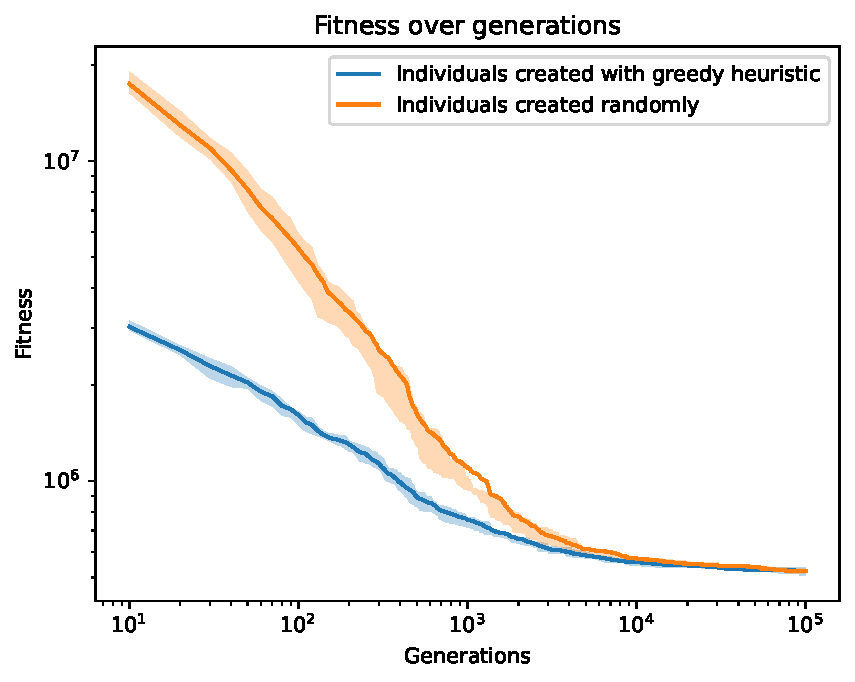
\includegraphics[width=\textwidth]{img/evo1_create_ind_random.pdf}
        \caption{Randomly distributed data}
        \label{fig:evo1_cind_random}
    \end{subfigure}
    \begin{subfigure}[b]{0.45\textwidth}
        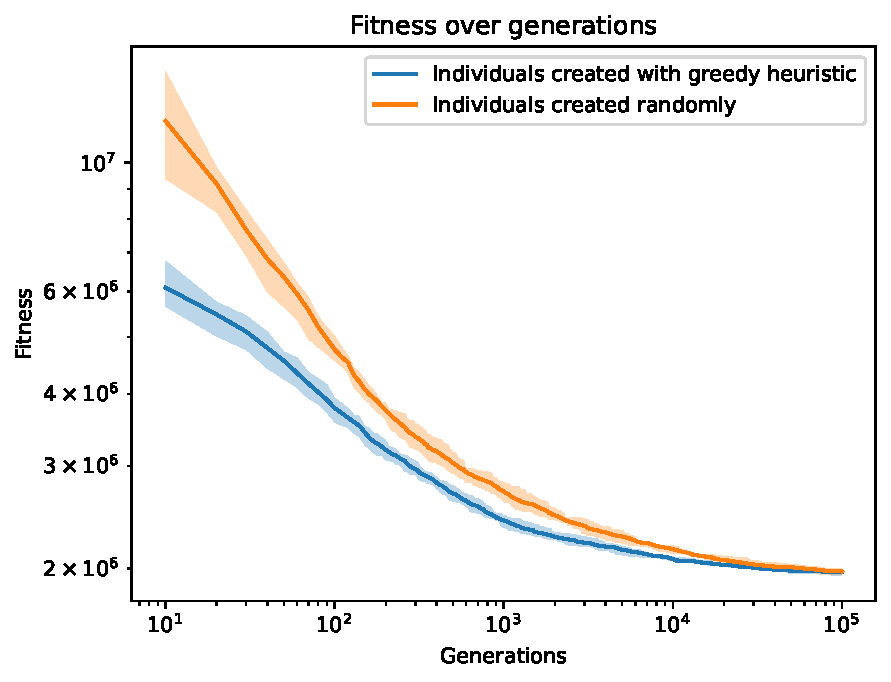
\includegraphics[width=\textwidth]{img/evo1_create_ind_commute.pdf}
        \caption{Long distance commute data}
        \label{fig:evo1_cind_commute}
    \end{subfigure}
    \caption{Individual as stops - population initialization}
    \label{fig:evo1_create_ind}
\end{figure}

\label{experiment_graph_description}
We will describe the experiments on the population initialization function. For both dataset types, we conduct two experiments, one with \textit{greedy} initialization and one with \textit{random} initialization. Both datasets are made of 50 customer requests, with group sizes between 1 and 10 persons and departure times in a 2-hour window. Each experiment runs the genetic algorithm 10 times. In figure \ref{fig:evo1_create_ind}, for each experiment, the mean fitness of the 10 runs is depicted as the primary line, accompanied by the first and third quartiles represented as a translucent region. Both $x$ and $y$ axes are logarithmic.

From the figure, we can see that for both datasets, the \textit{greedy} initialization resulted in faster convergence at the beginning. We therefore decided to use the \textit{greedy} initialization.

The rest of the hyper-parameter values were chosen similarly and are shown in the table \ref{tab:evo_stops_hyperparams}.

\begin{table}[ht]
    \centering
    \begin{tabular}{lc}
        Mutation probability & 0.8 \\
        Crossover probability & 0.2 \\
        Selection & tournament ($t=2$) \\
        Population size & 40 \\
        Create individual function & greedy \\
        Smart mutation weight & 12 \\
        Reverse a route weight & 3 \\
        Add/Delete/Change a stop randomly weight & 9 \\
        Shuffle individual weight & 2 \\
        Smart mutation maximum pick-up-drop-off distance & 20 \\
    \end{tabular}
    \caption{Individual as stops - hyper-parameter settings}
    \label{tab:evo_stops_hyperparams}
\end{table}

\subsection{Individual as separate clustering and routing}

The hyper-parameter settings for both dataset types were chosen experimentally and are shown in the table \ref{tab:evo_cr_hyperparams}.

\begin{table}[ht]
    \centering
    \begin{tabular}{lc}
        Mutation probability & 0.8 \\
        Crossover probability & 0.4 \\
        Selection & tournament ($t=2$) \\
        Population size & 30 \\
        Mutate route assignments probability & 0.5 \\
        Swap two groups between routes mutation probability & 0.5 \\
        Reverse a part of the order array mutation probability & 0.7 \\ 
    \end{tabular}
    \caption{Individual as cluster and route - hyper-parameter settings}
    \label{tab:evo_cr_hyperparams}
\end{table}

\subsection{Individual as only clustering with heuristic routing}

The hyper-parameter settings for both dataset types were chosen experimentally and are shown in the table \ref{tab:evo_ch_hyperparams}.

\begin{table}[ht]
    \centering
    \begin{tabular}{lc}
        Mutation probability & 0.8 \\
        Crossover probability & 0.3 \\
        Selection & tournament ($t=3$) \\
        Population size & 20 \\
        Travel time weight in heuristic cost & 1 \\
        Time window violation weight in heuristic cost & 2 \\
        Uniform crossover switch assignment probability & 0.2 \\
        Swap two groups between routes mutation probability & 0.5 \\
    \end{tabular}
    \caption{Individual as only clustering with heuristic routing - hyper-parameter settings}
    \label{tab:evo_ch_hyperparams}
\end{table}